\PassOptionsToPackage{english}{babel}
\documentclass{report}
\usepackage[utf8]{inputenc}

%\usepackage[english]{babel}
%\usepackage[latin1]{inputenc}
%\usepackage{geometry}
%\usepackage{listings}
\usepackage{caption}
\usepackage{amsmath}
\usepackage{graphics}
\usepackage[T1]{fontenc}
\usepackage{enumitem} %bold enumeration
\usepackage[utf8]{inputenc}
\usepackage[english]{babel}
%\usepackage{pmgraph}
\usepackage{mathrsfs}
\usepackage{floatflt}
\usepackage{multicol}
\usepackage{color,colortbl}
% \usepackage[pdftex]{graphicx}
\usepackage[normalem]{ulem}
\usepackage[colorlinks,urlcolor=blue, linkcolor=blue]{hyperref}
\usepackage{epstopdf}
\usepackage{wrapfig}
\usepackage{multirow}
%% Sets page size and margins
\usepackage[a4paper,top=3cm,bottom=2cm,left=3cm,right=3cm,marginparwidth=1.75cm]{geometry}
%% Useful packages
\usepackage[colorinlistoftodos]{todonotes}
\usepackage{xymtex}
\usepackage{fancyhdr}
\usepackage{epstopdf}
\usepackage{indentfirst} \geometry{verbose,a4paper,tmargin=3cm,bmargin=3cm,lmargin=1.0cm,rmargin=2.0cm}
\setlength{\parindent}{0pt}
\begin{document}
\large
Report of Anton Maksimov (antonma, 16-952-137), Task 10 "Image Categorization"\\
 on ETHZ course "Computer Vision".\\
\rule{\linewidth}{1pt}
%%%%%%%%%%%%%%%%%%%%%%%%%%%%%%%%%%%%%%%%%%%%%%%%%%%%%%%%%   1
	\textbf{Creating codebook.}\\
	 First we extract features from all training images just creating grid of $10\times10$ points and calculating HOG in $4\times4$ cells near this grid points by calculating histograms of gradient directions in $4\times4$ pixels in each of these cells. We use 8 bins for histograms, so map $[-\pi,\pi]$ to integers from 1 to 8 using division by $\pi/4+\epsilon$ ($\epsilon=10^{-10}$ in order to map $-2\pi$ correctly, without using special bin for it) and \texttt{floor} the result with shifting to positive integers by summing with 4. In order to have all pixels inside the image we create the grid with borders 8 pixels from each side. We concatenate all histograms from all cells to one array per grid point.
	 
	 Then, we cluster these arrays from all grid point from all training images using kmeans with $k$ clusters (fig. 1 \ref{codebook}). Later we vary this $k$ from $3$ to $1000$ (where results are good before dropping).\\
	 
	 \textbf{Bag of words}\\
	 To create bag of words we take testing images (separately positive and negative), extract patches as before, but then find the nearest in euclidean metric cluster center from codebook and add one to correspondent bin in bag-of-words (BoW) histogram for each training image. So, we have positive (PosBoW) and negative (NegBoW) sets of histograms.\\
	  
	 \textbf{Classification}\\
	 \textsc{Nearest neighbor}\\
	 For each testing image we use \texttt{knnsearch} to find nearest BoW of negative and positive training images, and then assign positive label, if distance to the nearest positive one is less than to the negative one.
	 \\
	 
	 \textsc{Bayesian}\\
	 We model distributions of histograms for one Word in PosBoW and NegBoW as normal with inferred mean and std of the extracted empirical ones. Then we assume all these words to be independent and model probability of being our image positive from Bayes' formula assuming prior probability to find a car as 0.5. Because small probabilities multiplied many times can lead to numerical instabilities, we calculate sum of natural logarithms of pdfs calculated in point --- number of appearances of the word in this particular image, when pdf's mean and std are taken from correspondent positive or negative distributions in testing images.
	 
	 Also, in order to avoid NaNs we skip in the sum words which have zero mean and std.
	 
	 As a result, assuming denominator not zero in Bayes' formula (it's almost impossible with normal images), we compare numerators for positive and negative variants and choose the biggest one's variant (negative if equal).\\
	 
	 \textbf{Results}\\
	 We obtain fraction of rightly classified training images, repeating the algorithm for 10 times (then better quality of statistics) for different size of codebook (see the table \ref{table}) (full results in .xlsx file in results folder).
	 
	 As can be seen from results (fig. 2 \ref{comp}), in provided dataset nearest neighbor classification algorithm works more stable in wider range and comparable with Bayesian one + it has less fluctuation. But Bayesian is better with small number of words (even the best is with 5-10 words), because these are the most significant, but nearest neighbor is worse there because of too small density of centers in space, so it's more usual to assign to far centers, which have lesser common with current image). 
	 
	 Bayesian approach doesn't work with big number of words because then there are less appearances of one word and less of them could be approximated as normal (because normal model, probably, comes from the law of big numbers, when there are big numbers in histograms).\\
	 
	 In general, we can't say that one approach is better than another from our results, because among sizes of codebook where both work the best, their difference is insignificant due to estimated variance.\\
	 
	 \textbf{Bonus}\\
	 Also, we collected in Zurich and Dietikon our own dataset (\href{https://drive.google.com/drive/folders/1rt7VSSvhPKGTcGuDaD1_le7s5Z9yq1aX?usp=sharing}{google disk}) of images of cars <<in profile>> as positives and images of road and surroundings as negatives (60 images --- for 15 in each of positive--negative and training--test). In order to compare with provided dataset we resize images to  to comparable size (10 times less in each dimension from $3928\times 2208$). Other parameters are the same. (we changed names of folders in \texttt{bow\_evaluation.m}, and ".png" to ".jpg" plus  resized images in \texttt{create\_bow\_histograms.m} and \texttt{create\_codebook.m}.
	 
	 Because this dataset is smaller, variance of results is bigger, in general (discretization error (due to discrete possible values of resulting ratio) was $1/100/2 = 0.005$ before, now it' $1/30/2 \approx 0.015$ only because of the smaller number of data). Also, results for Bayesian labeling are better, because, maybe, it's more uniform dataset, so distribution among histograms is better modeled with Gaussians. Plus, images are of a better quality even after resizing. (fig 3\ref{comp2}, table \ref{table1})
	

\begin{figure}[h]
	\begin{center}
		\label{codebook}
		\begin{minipage}[h]{0.3\linewidth}
			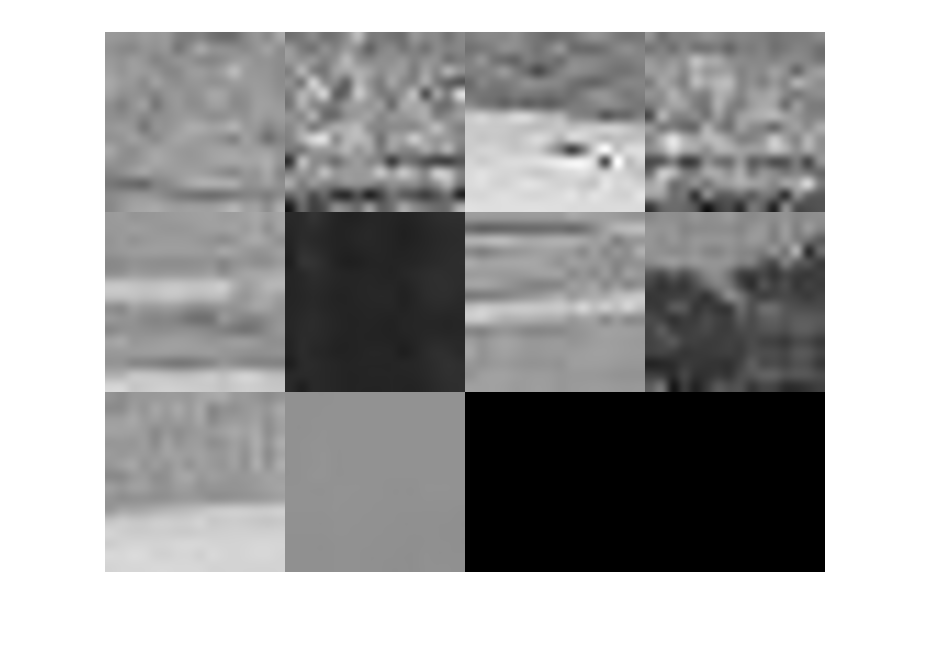
\includegraphics[width=1\linewidth]{C:/Users/Anton/Desktop/ETH_books/CV/cv_lab10_image_categorization/results/codebook_k=10}
		\end{minipage}
		\hfill
		\begin{minipage}[h]{0.3\linewidth}
			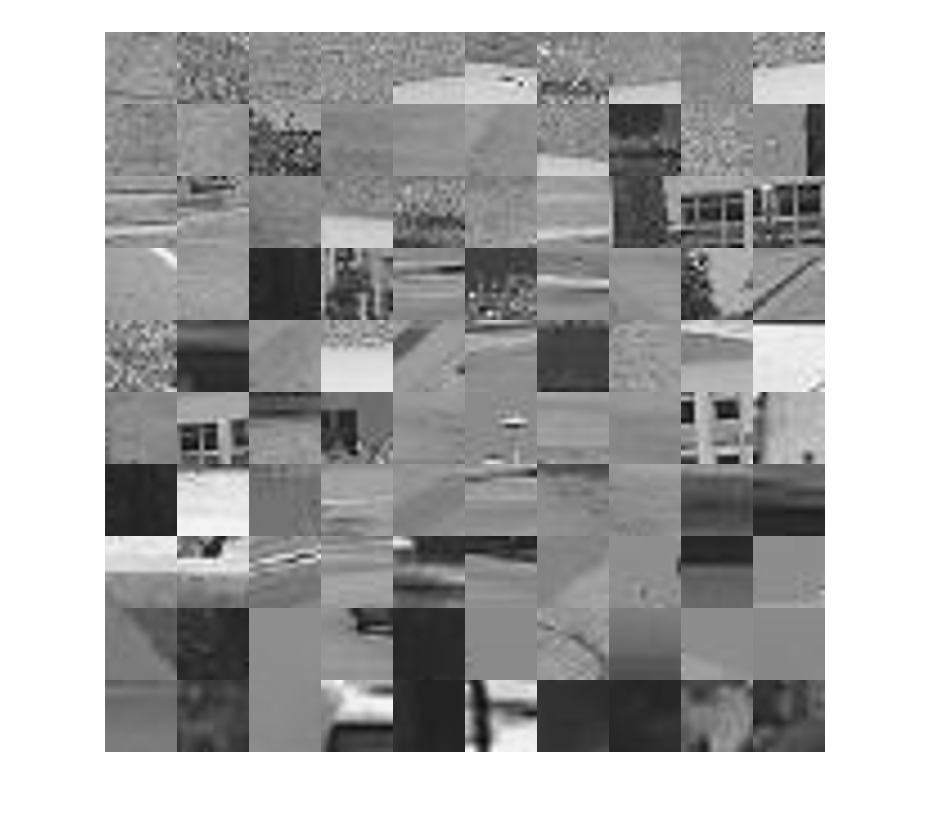
\includegraphics[width=1\linewidth]{C:/Users/Anton/Desktop/ETH_books/CV/cv_lab10_image_categorization/results/codebook_k=100}
		\end{minipage}
		\hfill
		\begin{minipage}[h]{0.3\linewidth}
			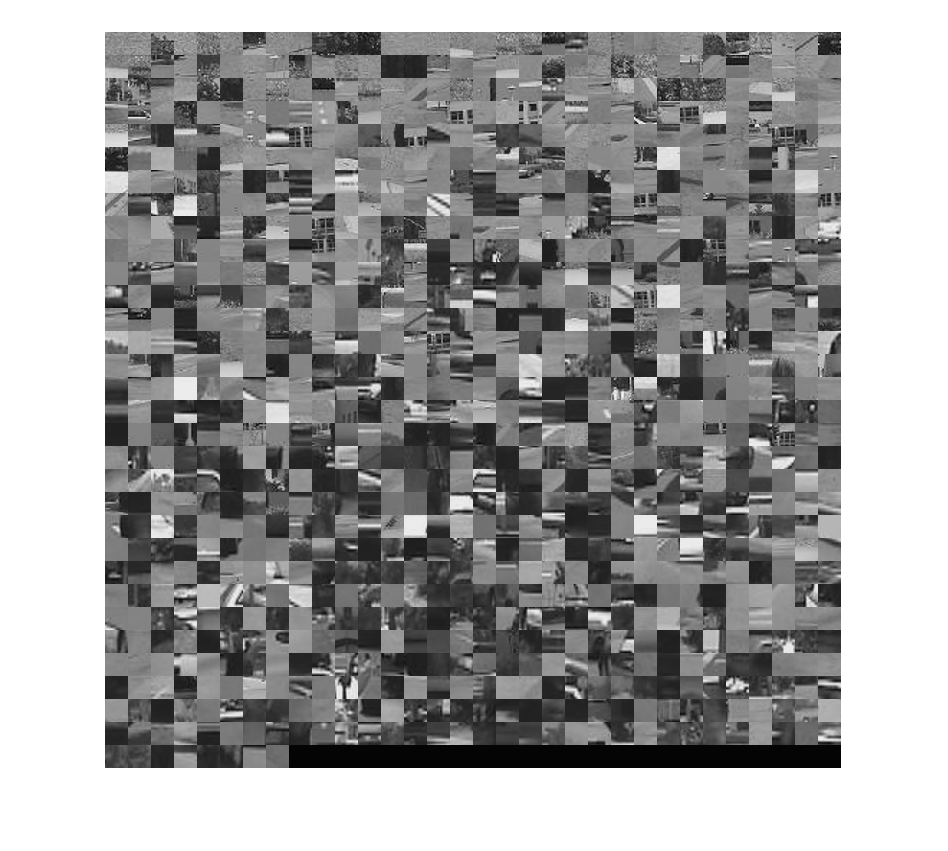
\includegraphics[width=1\linewidth]{C:/Users/Anton/Desktop/ETH_books/CV/cv_lab10_image_categorization/results/codebook_k=1000}
		\end{minipage}
		\caption{Codebooks for 10, 100 and 1000 patches (black squares in the last line are just filling, it's not extracted patches).}
	\end{center}
\end{figure}

\begin{figure}[h!]
	
	\begin{center}
		
		\begin{minipage}[h]{0.95\linewidth}
			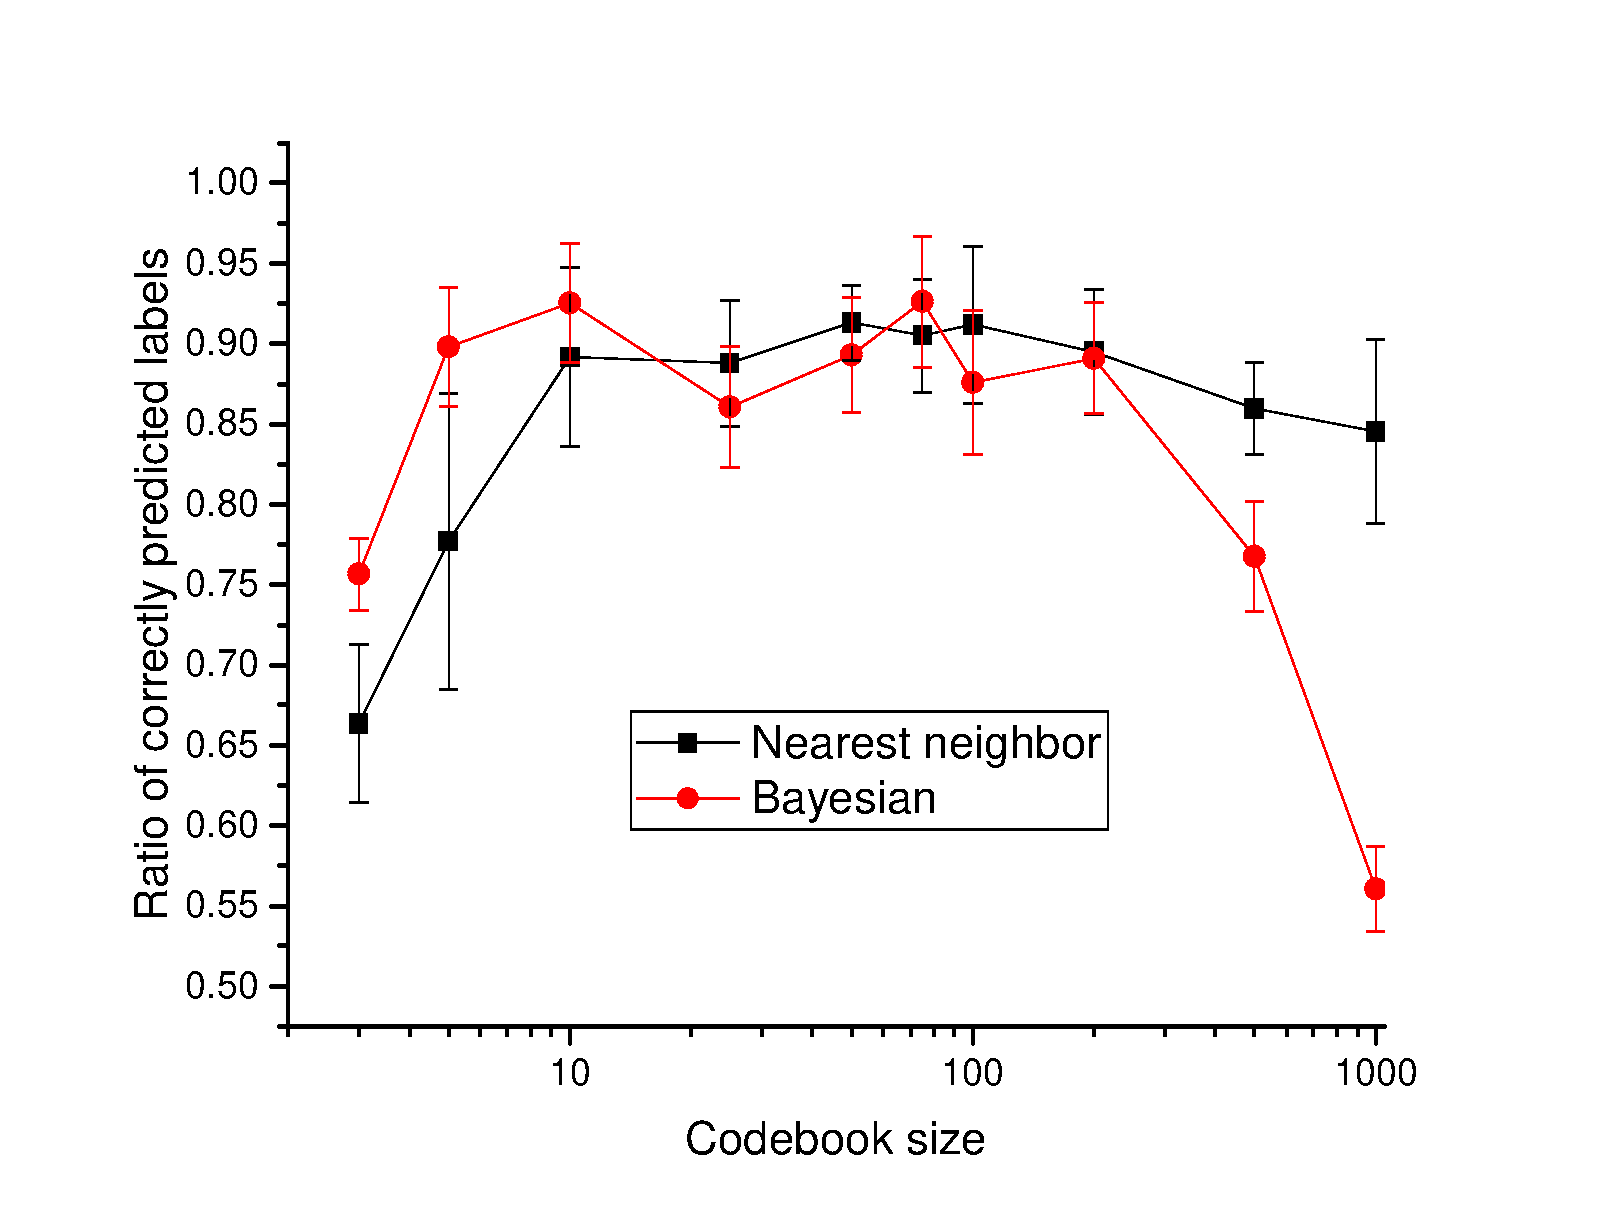
\includegraphics[width=1\linewidth]{C:/Users/Anton/Desktop/ETH_books/CV/cv_lab10_image_categorization/results/Graph1}
		\end{minipage}
		
		\caption{Results for two types of label assigning for provided dataset.}
	\end{center}
\label{comp}
\end{figure}

% Please add the following required packages to your document preamble:
% \usepackage{multirow}
\centering

\begin{table}[]
	\caption{Results for provided dataset}
	\label{table}
	\begin{center}
	\begin{tabular}{|l|l|l|l|l|}
		\hline
		\multicolumn{1}{|c|}{\multirow{2}{*}{\begin{tabular}[c]{@{}c@{}}Codebook\\ size\end{tabular}}} & \multicolumn{2}{l|}{Nearest neighbor} & \multicolumn{2}{l|}{Bayesian} \\ \cline{2-5} 
		\multicolumn{1}{|c|}{}                                                                         & mean              & std               & mean          & std           \\ \hline
		10                                                                                             & 0.89193           & 0.05588           & 0.92526       & 0.037302      \\ \hline
		25                                                                                             & 0.88789           & 0.039493          & 0.86062       & 0.037737      \\ \hline
		50                                                                                             & 0.91314           & 0.023557          & 0.89294       & 0.035908      \\ \hline
		75                                                                                             & 0.90506           & 0.035336          & 0.92627       & 0.040664      \\ \hline
		100                                                                                            & 0.91213           & 0.048868          & 0.87577       & 0.044726      \\ \hline
		200                                                                                            & 0.89496           & 0.038908          & 0.89092       & 0.034636      \\ \hline
		500                                                                                            & 0.85961           & 0.02837           & 0.7677        & 0.034102      \\ \hline
		1000                                                                                           & 0.84547           & 0.057143          & 0.56065       & 0.026434      \\ \hline
	\end{tabular}
\end{center}
\end{table}

\begin{figure}[h!]
	
	\begin{center}
		
		\begin{minipage}[h]{0.95\linewidth}
			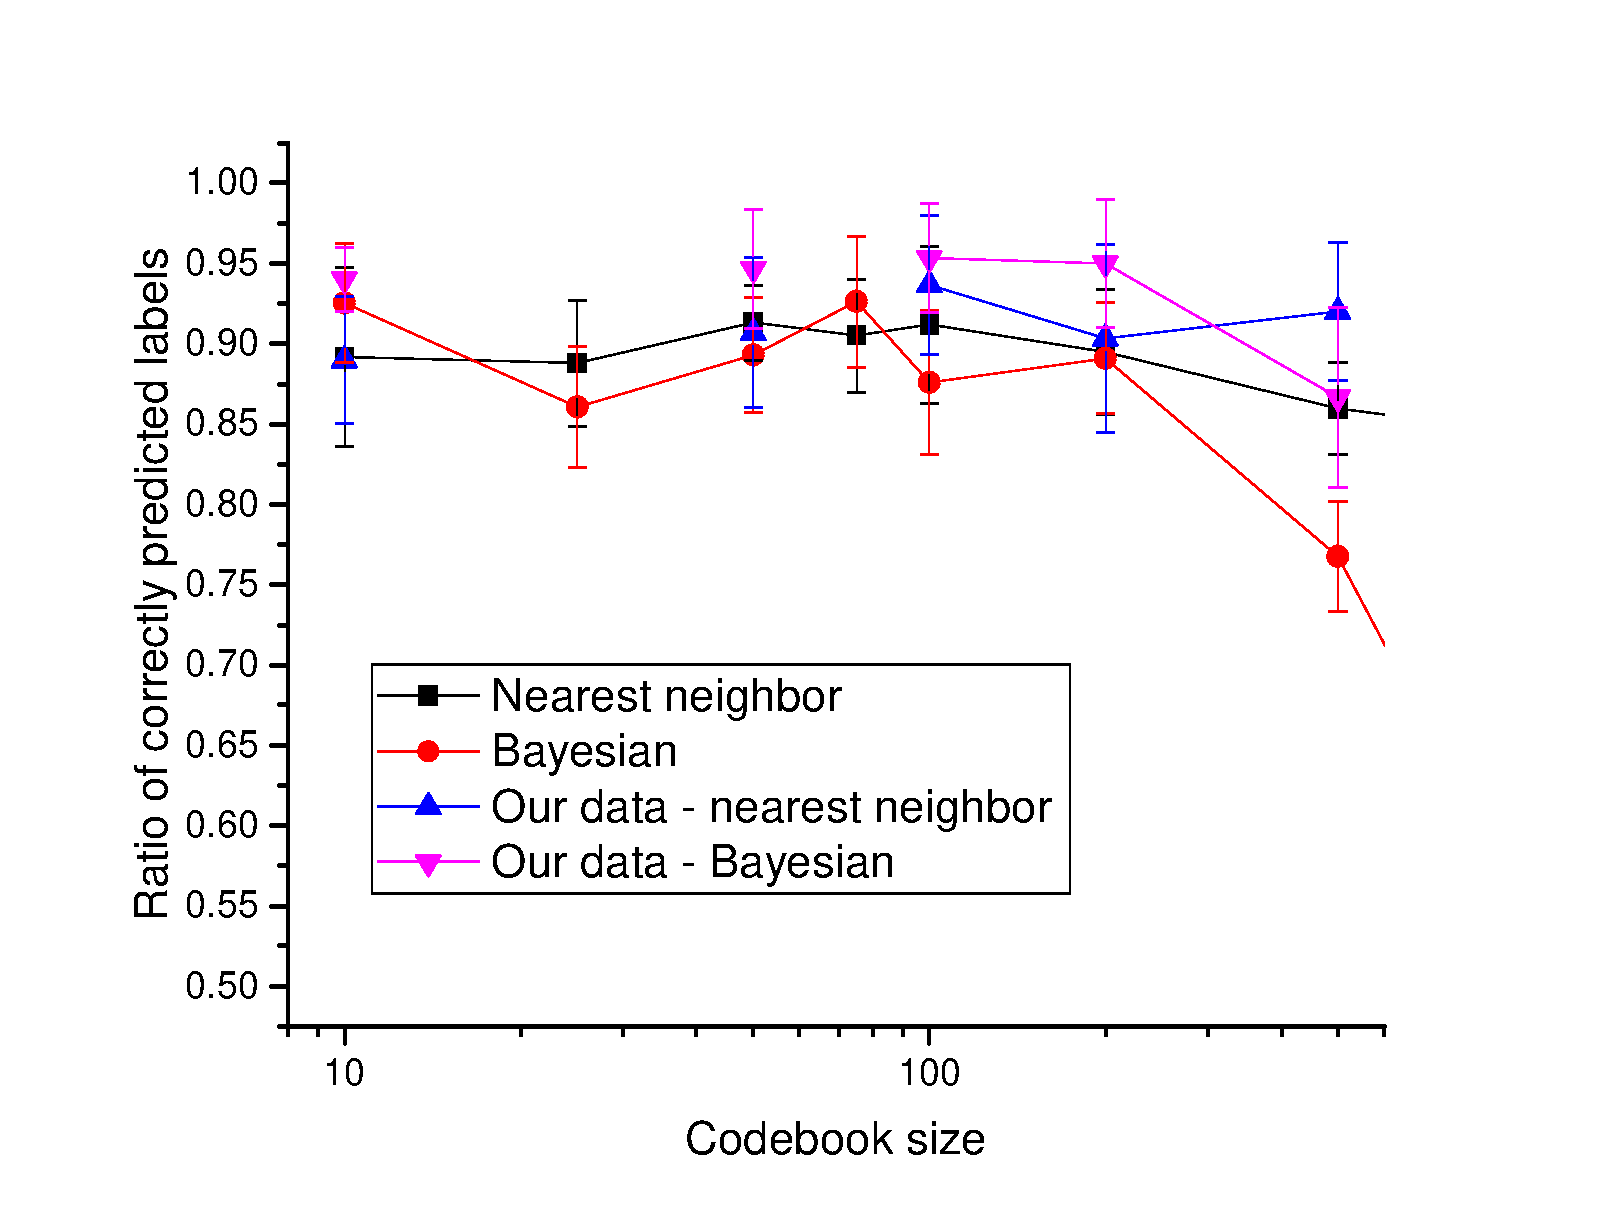
\includegraphics[width=1\linewidth]{C:/Users/Anton/Desktop/ETH_books/CV/cv_lab10_image_categorization/results/Graph2}
		\end{minipage}
		
		\caption{Results for two types of label assigning for self-obtained and provided dataset.}
	\end{center}
	\label{comp2}
\end{figure}

% Please add the following required packages to your document preamble:
% \usepackage{multirow}
\begin{table}[]
	\caption{Results for self-obtained dataset}
	\label{table1}
		\begin{center}
	\begin{tabular}{|l|l|l|l|l|}
		\hline
		\multicolumn{1}{|c|}{\multirow{2}{*}{\begin{tabular}[c]{@{}c@{}}Codebook\\ size\end{tabular}}} & \multicolumn{2}{l|}{Nearest neighbor} & \multicolumn{2}{l|}{Bayesian} \\ \cline{2-5} 
		\multicolumn{1}{|c|}{}                                                                         & mean              & std               & mean          & std           \\ \hline
		10                                                                                             & 0.89001           & 0.039575          & 0.93999       & 0.02002       \\ \hline
		50                                                                                             & 0.90667           & 0.046669          & 0.94668       & 0.037123      \\ \hline
		100                                                                                            & 0.93667           & 0.043333          & 0.95334       & 0.034003      \\ \hline
		200                                                                                            & 0.90335           & 0.058592          & 0.95001       & 0.04014       \\ \hline
		500                                                                                            & 0.91999           & 0.042695          & 0.86667       & 0.055763      \\ \hline
	\end{tabular}
\end{center}
\end{table}
\end{document}
